% The mush model: a fin and the PCM in the half-gap beside it, at one position along the tube
\documentclass[tikz, border=4pt]{standalone}
% Shared preamble of the PyTES model diagrams: packages, colours and styles.
% Each diagram is a standalone document that inputs this file; build them with build.py.
\usepackage{amsmath}
\usepackage{bm}
\usetikzlibrary{arrows.meta, calc, decorations.pathreplacing, patterns, positioning}

% The PyTES Thermal colour cycle (pytes.plotting.THERMAL) and tints of it
\definecolor{pytesorange}{HTML}{E8590C}
\definecolor{pytesblue}{HTML}{1F4E9C}
\definecolor{pytesteal}{HTML}{14A08A}
\definecolor{pytesamber}{HTML}{F0A930}
\definecolor{pytesplum}{HTML}{A23B72}
\definecolor{pytessky}{HTML}{88C7F0}
\definecolor{pytesink}{HTML}{36312E}

% Materials: the heat transfer fluid, the PCM, the metal (fins and tubes)
\colorlet{fluidfill}{pytessky!75}
\colorlet{pcmfill}{pytesamber!55}
\colorlet{liquidfill}{pytesorange!60}
\colorlet{metalfill}{pytesink!45}
\colorlet{compositefill}{pcmfill!85!metalfill}

\tikzset{
  >={Stealth[length=2.2mm]},
  every picture/.style={line join=round, line cap=round, font=\small},
  outline/.style={draw=pytesink, line width=0.6pt},
  fluid/.style={outline, fill=fluidfill},
  pcm/.style={outline, fill=pcmfill},
  liquid/.style={outline, fill=liquidfill},
  metal/.style={outline, fill=metalfill},
  composite/.style={outline, fill=compositefill},
  flow/.style={->, draw=pytesblue, line width=1.2pt},
  heat/.style={->, draw=pytesorange, line width=1.1pt},
  axis/.style={->, draw=pytesink, line width=0.7pt},
  dimension/.style={<->, >={Stealth[length=1.6mm]}, draw=pytesink, line width=0.5pt},
  guide/.style={draw=pytesink!60, line width=0.4pt, dashed},
  symmetry/.style={draw=pytesink, line width=0.5pt, dash dot},
  label/.style={text=pytesink, font=\small},
  note/.style={text=pytesink, font=\footnotesize, align=center},
}

\begin{document}
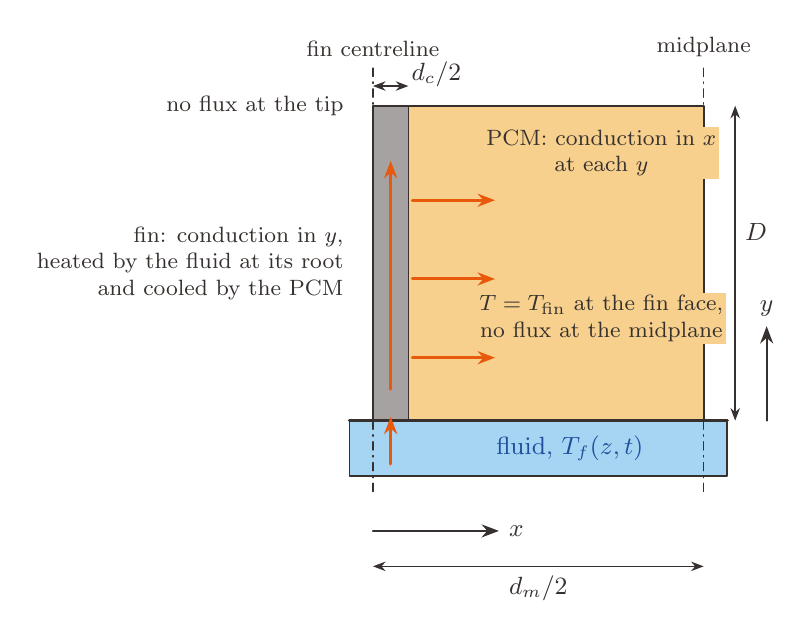
\begin{tikzpicture}
  \def\fin{0.45}   % half the fin thickness, d_c / 2
  \def\gap{4.2}    % half the fin pitch, d_m / 2
  \def\Rf{0.0}
  \def\D{4.0}
  % Fluid along the wall, the fin, the PCM
  \draw[fluid] (-0.3, -0.7) rectangle (\gap + 0.3, \Rf);
  \draw[metal] (0, \Rf) rectangle (\fin, \Rf + \D);
  \draw[pcm] (\fin, \Rf) rectangle (\gap, \Rf + \D);
  \draw[outline, line width=1.1pt] (-0.3, \Rf) -- (\gap + 0.3, \Rf);
  \draw[symmetry] (0, \Rf - 0.9) -- (0, \Rf + \D + 0.5);
  \draw[symmetry] (\gap, \Rf - 0.9) -- (\gap, \Rf + \D + 0.5);
  \node[note, anchor=south] at (0, \Rf + \D + 0.5) {fin centreline};
  \node[note, anchor=south] at (\gap, \Rf + \D + 0.5) {midplane};
  \node[label, text=pytesblue] at (\gap/2 + 0.4, \Rf - 0.35) {fluid, $T_f(z, t)$};
  % Heat paths: fluid to fin root, along the fin, into the PCM
  \draw[heat] (\fin/2, \Rf - 0.55) -- (\fin/2, \Rf + 0.05);
  \draw[heat] (\fin/2, \Rf + 0.4) -- (\fin/2, \Rf + 3.3);
  \foreach \yc in {0.8, 1.8, 2.8} {
    \draw[heat] (\fin + 0.05, \yc) -- (\fin + 1.1, \yc);
  }
  \node[note, fill=pcmfill, inner sep=1pt, align=center] at (2.9, 3.4)
    {PCM: conduction in $x$\\at each $y$};
  \node[note, fill=pcmfill, inner sep=1pt, align=center] at (2.9, 1.3)
    {$T = T_\mathrm{fin}$ at the fin face,\\no flux at the midplane};
  \node[note, anchor=east, align=right] at (-0.25, 2.0)
    {fin: conduction in $y$,\\heated by the fluid at its root\\and cooled by the PCM};
  \node[note, anchor=east, align=right] at (-0.25, \Rf + \D) {no flux at the tip};
  % Coordinates and dimensions
  \draw[axis] (\gap + 0.8, \Rf) -- (\gap + 0.8, \Rf + 1.2) node[label, above] {$y$};
  \draw[axis] (0, -1.4) -- (1.6, -1.4) node[label, right] {$x$};
  \draw[dimension] (0, \Rf + \D + 0.25) -- (\fin, \Rf + \D + 0.25);
  \node[label, anchor=south west, inner sep=1pt] at (\fin, \Rf + \D + 0.2) {$d_c / 2$};
  \draw[dimension] (0, -1.85) -- (\gap, -1.85) node[label, midway, below] {$d_m / 2$};
  \draw[dimension] (\gap + 0.4, \Rf) -- (\gap + 0.4, \Rf + \D)
    node[label, pos=0.6, right] {$D$};
\end{tikzpicture}
\end{document}
